\section{Experimental Evaluation}
Each of our aforementioned goals has a different metric
for success, thus we conducted a performance-based
analysis of our simulator and replay tool and a
qualitative/correctness-oriented evaluation for
VAPP's parallel program analysis components.  The achievement
of our goal to allow users to easily view and
interact with their applications' traces is demonstrated
in Figures \ref{pic:sqlite_browse} and \ref{pic:sqlite_query}
and did not warrant further evaluation.

\subsection{Simulator Performance}
\label{sec:sim_perf}

\begin{figure}
  \lstset{language=C, basicstyle=\small}
  \begin{lstlisting}
#define N 200

int main(void){
  int value = 0xCafeBabe;
  int *buffer;
  int i = 0;

  buffer = (int*)malloc(N*N*sizeof(int));

  for ( i = 0 ; i < N*N ; i++ ) {
      buffer[i] = value;
  }

  return buffer[0];
}
  \end{lstlisting}
  \caption{The source code for \texttt{test\_init} program. (Note the memory leak is intentional.)}
  \label{fig:test_init}
\end{figure}

As one of our goals was to provide a fast replay mechanism for the
logged data. We developed, based on the cache simulator from our
$1^{st}$ assignment (hereafter referred to as \emph{scs\_pin}), a cache
simulator that uses our replay mechanism (hereafter referred to as
\emph{scs\_replay}). Given the fact that our pin version of the cache
simulator already used the Executor abstraction, the port was straightforward
and allowed us to compare functionally and implementation-wise
completely identically cache simulators with each other. To evaluate
the performance we wrote a simple benchmark program (see Figure
\ref{fig:test_init}) that initializes a memory array. We then evaluated
and compared the two following approaches by varying the parameter N:

\begin{description}
  \item[scs\_pin] Run the benchmark application with the Pin version of
    our cache simulator.
  \item[scs\_replay] First run the benchmark application with our Pin
    tool to gather a trace file. Then use this trace file as the
    source for our replay library.
\end{description}

\begin{table*}
  \begin{tabularx}{\textwidth}{X r r r r r}
    \toprule
    Program/Configuration & Time (no logging) [s] & Time (logging) [s] & log size [bytes] & scs\_relay [s] & scs\_pin [s]\\
    \midrule
    %% helloword         & 1.21 & 12.14 &  6961152 & 0.70  & 0.89 \\
    \addlinespace[1mm]
    \rowcolor[gray]{.9}
    test\_init/N=10   & 1.23 & 11.48 &  6601728 & 0.66 & 0.89 \\
    \addlinespace[1mm]
    test\_init/N=20   & 1.23 & 11.48 &  6717440 & 0.66 & 0.89 \\ 
    \addlinespace[1mm]
    \rowcolor[gray]{.9}
    test\_init/N=30   & 1.25 & 12.07 &  6912000 & 0.70 & 0.90 \\
    \addlinespace[1mm]
    test\_init/N=40   & 1.24 & 12.57 &  7183360 & 0.74 & 0.90 \\
    \addlinespace[1mm]
    \rowcolor[gray]{.9}
    test\_init/N=50   & 1.25 & 13.19 &  7532544 & 0.76 & 0.90 \\
    \addlinespace[1mm]
    test\_init/N=100  & 1.24 & 18.71 & 10441728 & 1.08 & 0.90 \\
    \addlinespace[1mm]
    \rowcolor[gray]{.9}
    test\_init/N=150  & 1.26 & 27.79 & 15292416 & 1.60 & 0.90 \\
    \addlinespace[1mm]
    test\_init/N=200  & 1.28 & 40.57 & 22071296 & 2.33 & 1.04 \\
    \bottomrule
  \end{tabularx}
  \caption{Performance evaluation and comparison of the cache
    simulator using the Pin infrastructure directly and using our
    replay library.}
  \label{tbl:results}
\end{table*}

Table \ref{tbl:results} summaries the results from our
evaluation. Note that there is a change of the stepping. While the
first 4 runs increase N by 10, the last 4 runs increased N by 50. The
following section will discuss these results in more detail.

\begin{figure}
  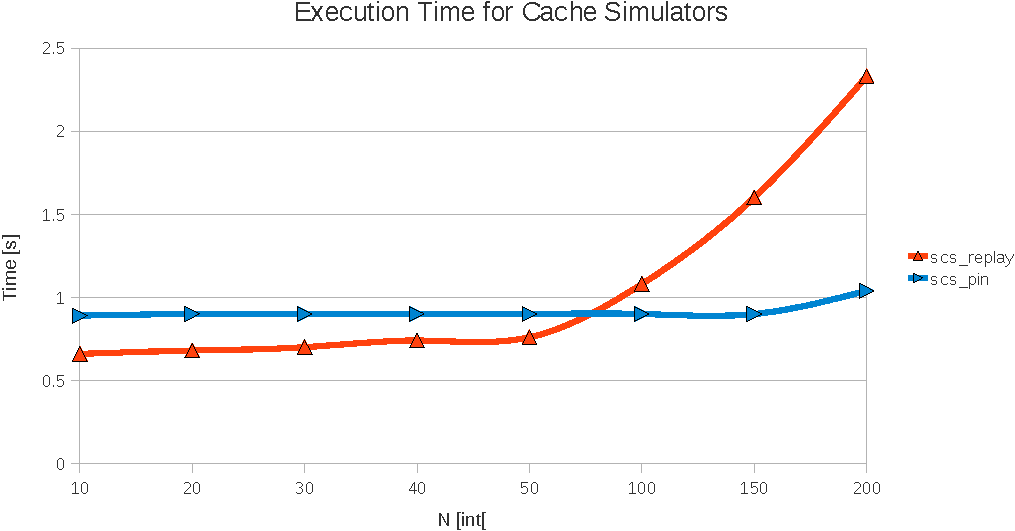
\includegraphics[width=\columnwidth]{eval_execution_time_replay}
  \caption{The execution time of the cache simulator using the Pin
    infrastructure or our replay library.}
  \label{fig:eval_execution_time_replay}
\end{figure}

As one of our main goals was to provide a faster way of performing analysis,
our main interest was the comparison of the cache simulator execution
times. As shown in Figure \ref{fig:eval_execution_time_replay}, the
execution time for the replay version (scs\_replay column in the table) is only better 
than for the `native' Pin tool version (scs\_pin column) for very small N.
As soon as N gets bigger than
100, we can see a clear trend towards a drastic performance penalty
for our replay approach. In the next section we will break down our
analysis of this phenomenon.

\begin{figure}
  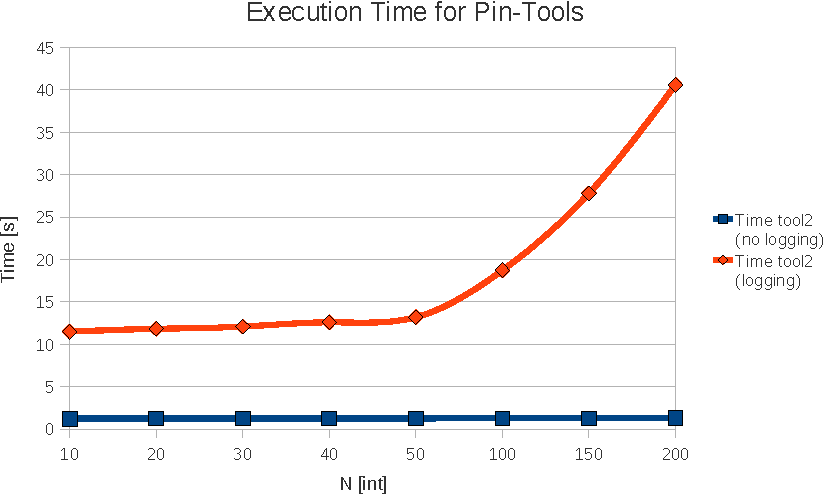
\includegraphics[width=\columnwidth]{eval_execution_time_tracing}
  \caption{The execution time of our tracing generator, comparing the
    case where actual data is written and the case where we just run
    the application without performing any log operations.}
  \label{fig:eval_execution_time_tracing}
\end{figure}

\begin{figure}
  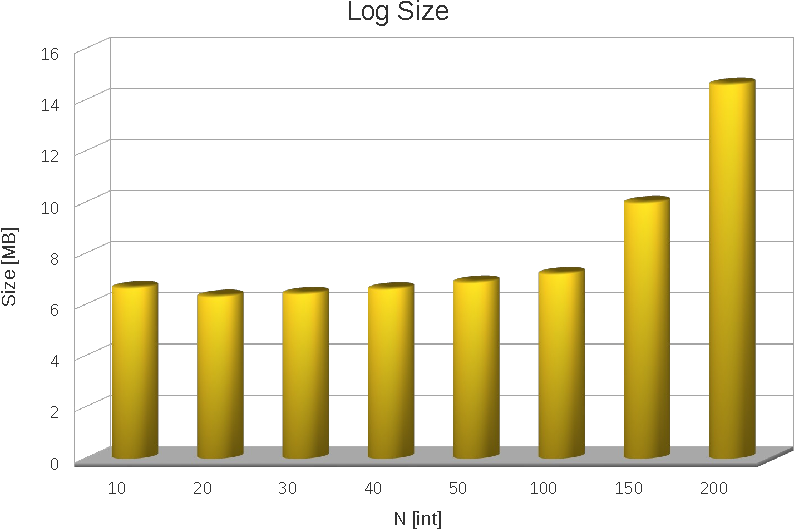
\includegraphics[width=\columnwidth]{eval_log_size}
  \caption{The growth of the log size while changing parameter N of the \texttt{test\_init} program. }
  \label{fig:eval_log_size}
\end{figure}


While gathering the tracing information we already realized a
performance hit. To get an better understanding of the possible
performance costs of the SQLite database we compared the dry-run mode
of our Pin tool, which does not write any logging information, with
the normal mode of our Pin tool. The results are shown Figure
\ref{fig:eval_execution_time_tracing}. As seen in the figure, the
execution time for the case without writing any logging information
performs almost linearly as N grows, while execution with writing logging
information is at least one order of magnitude worse (with a trend
that appears to be exponential). A reason for this behavior can be directly 
inferred by observing the amount of data that is stored in the
database, as shown in Figure \ref{fig:eval_log_size}\footnote{Note
  that the store operations modify a database table and do not just
  append the file.}. The execution time of the Pin tool is dominated
by the increasing I/O costs as N grows, and the execution time
and log size exhibit the same trend.
   
To confirm this observation and evaluate if there
is a single root cause that we could potentially overcome, recompiled
the whole software stack with profiling information and re-ran the
replay cache simulator with the input for N = 200. As shown in
Figure \ref{fig:profiler}, almost half of the time is spent by
an internal SQLite function, converting the data from the database
into a string representation.


\begin{figure*}
  \lstset{basicstyle=\footnotesize, mathescape=true}
  \begin{lstlisting}
Each sample counts as 0.01 seconds.
  %   cumulative   self              self     total           
 time   seconds   seconds    calls  ms/call  ms/call  name    
 43.44      0.43     0.43  4047013     0.00     0.00  sqlite3VXPrintf
 12.12      0.55     0.12   809419     0.00     0.00  sqlite3VdbeExec
  6.06      0.61     0.06   758517     0.00     0.00  Profiler::addToRead(long, long, long, long)
  3.03      0.64     0.03  5665887     0.00     0.00  sqlite3ApiExit
  3.03      0.67     0.03  4047031     0.00     0.00  sqlite3ValueText
  3.03      0.70     0.03  4047017     0.00     0.00  sqlite3StrAccumAppend
  3.03      0.73     0.03   809305     0.00     0.00  Profiler::addToUsage(long, long)
  2.53      0.76     0.03  4047023     0.00     0.00  sqlite3VdbeSerialGet
  2.02      0.78     0.02  4047031     0.00     0.00  sqlite3VdbeChangeEncoding
  2.02      0.80     0.02  4047023     0.00     0.00  columnMem
  2.02      0.82     0.02  4047012     0.00     0.00  sqlite3_snprintf
  2.02      0.84     0.02   809401     0.00     0.00  callback(void*, int, char**, char**)
  1.52      0.85     0.02  4047059     0.00     0.00  sqlite3DbMallocSize
  $\vdots$
  \end{lstlisting}
  \caption{GProf results of the cache simulator run using our replay library}
  \label{fig:profiler}
\end{figure*}


To put our log size into context, we compared VAPP's logs with those
from several related systems discussed in Section \ref{sec:intro}.
Note that the following results were reported by the respective authors;
we did not conduct these tests ourselves.
SIGMA employs sophisticated compression techniques before writing
its trace file, however the effectiveness of the compression is
heavily dependent on the program that is executed.  In some cases
a several hundred MB trace was compressed to less than 1 MB,
but in the worst case SIGMA's log files were several hundred MB
large \emph{after} compression.  Note however that the SIGMA benchmarks
were run on more complex programs than \texttt{test\_init} and that
VAPP's log files would likely grow to this magnitude or more if
run on identical benchmarks.

FDR and BugNet log files were measured after recording a 1 billion
instruction replay window.  FDR's log was only 34 MB, which is vastly
less than what VAPP would generated if tracing a 1 billion instruction
program.  However, recall that FDR utilizes advanced hardware support and
compression, and also requires a full memory dump in addition to the
reasonably sized log file.  BugNet only logs load values, thus on average
its log file was less than 20 MB during testing.  In the worst case
benchmark, it grew to over 100 MB.  The fact that VAPP's log for a
simple benchmark is roughly the same size as BugNet's for a 1 billion
instruction window indicates that detailed logging requires advanced
compression methods in order to scale.


\subsection{Concurrency Analysis Results}

%% \begin{figure}
%%   \centering
%%   \lstset{language=C, basicstyle=\small}
%%   \subfloat{
%%     \begin{minipage}{.4\textwidth}
%%       \begin{lstlisting}
%% %% int main(void) 
%% %% {
%% %%   int *result = (int*)malloc(sizeof(int));
%% %%   int value = 3;
  
%% %% #pragma omp parallel for 
%% %%   for ( int i = 0 ; i < 100  ; i++ )  {
%% %%     if ( i % value == 0) {
%% %%       #pragma omp critical 
%% %%       {
%% %%         if ( *result < i ) {
%% %%           *result = i;
%% %%         }
%% %%       }
%% %%     }
%% %%   }
%% %% }
%%       \end{lstlisting}
%%     \end{minipage}
%%     }
%%   \caption{The source code for \texttt{test\_openmp} program.}
%%   \label{fig:test_openmp}
%% \end{figure}


As described in Section \ref{sec:ppa}, we shifted our focus towards
the analysis of concurrent programs. Here we present the
a short evaluation of our second analysis. In Figure \ref{fig:openmp}
a short test Open MP program is shown. While the left version of the
program has a race condition, by not correctly synchronizing the access
to the result buffer, the version on the right side correctly uses a
critical section to protect access to the result buffer.

Below the source code of the programs the output of VAPP's extended
analysis is shown\footnote{We ran this test on a dual core
  machine.}. First the analysis prints the threads along with their
accesses buffers. Then it prints for every shared buffer the
lockset of the each thread\footnote{Note that the addresses of the
  buffers may differ between different runs, depending on the address
  that is returned by malloc.}. As shown on the analysis for the
incorrect version, none of the 3 shared buffers are protected by a
lock. In the correctly synchronized version we can see that the
lockset of the first shared buffer is not empty and in fact we realize
that this buffer is locked by the internal lock of the Open MP library
(indicated by the magic value, as described in Section \ref{sec:ppa}).

In both cases we see buffers that are shared and not protected by any
locks. Those are internal buffers of Open MP. Given our current
implementation, our analysis has the disadvantage that
if a buffer is accessed without any protecting lock being held, then
the resulting lockset will always be empty. This is phenomena appears
if for instance one thread allocates the buffer and initializes the
buffer without holding a lock. Future work could extend the current
analysis to employ heuristics to detect when a buffer leaves the
thread local state and enters the shared and vice versa, possibly by
extending Eraser's approach to a similar problem \cite{savage1997eraser}

% Decided not to include slowdown since we didn't explicilty measure it

%FDR, claims 2\% slowdown in a typically scenario
%Programs run 10 to 30 times slower with Eraser.
%MemSpy results in 22 to 58 times slowdown during testing on a single processor.

\begin{figure*}
  \centering
  \lstset{language=C, basicstyle=\small}

  \begin{minipage}{.45\textwidth}
    \begin{lstlisting}
int main(void) 
{
  int *result = (int*)malloc(sizeof(int));
  int value = 3;
  
#pragma omp parallel for 
  for ( int i = 0 ; i < 100  ; i++ )  {
    if ( i % value == 0) {
      if ( *result < i ) {
        *result = i;
      }
    }
  }
}
    \end{lstlisting}
    \vspace{8mm}
    \lstset{basicstyle=\scriptsize}
    \begin{lstlisting}
== ANALYSE =======================================
Thread 0 -> [11018256,11018288,11019872,11020080]>
Thread 1 -> [11018256,11018288,11019872]>
shared buffer 11018256
  t1 []
  t2 []
shared buffer 11018288
  t1 []
  t2 []
shared buffer 11019872
  t1 []
  t2 []
    \end{lstlisting}
  \end{minipage}
  \hspace{.025\textwidth}
  \hspace{.025\textwidth}
  \begin{minipage}{.45\textwidth}
    \begin{lstlisting}
int main(void) 
{
  int *result = (int*)malloc(sizeof(int));
  int value = 3;
  
#pragma omp parallel for 
  for ( int i = 0 ; i < 100  ; i++ )  {
    if ( i % value == 0) {
      #pragma omp critical 
      {
        if ( *result < i ) {
          *result = i;
        }
      }
    }
  }
}
    \end{lstlisting}
    \lstset{basicstyle=\scriptsize}
    \begin{lstlisting}
== ANALYSE =======================================
Thread 0 -> [32243728,32243760,32245344,32245552]>
Thread 1 -> [32243728,32243760,32245344]>
shared buffer 32243728
  t1 [666]>
  t2 [666]>
shared buffer 32243760
  t1 []
  t2 []
shared buffer 32245344
  t1 []
  t2 []
    \end{lstlisting}
  \end{minipage}
  \caption{Comparison of an incorrect (left) and a correct (right)
    Open MP program, along with the results of out analysis.}
  \label{fig:openmp}
\end{figure*}